\documentclass[10pt,landscape]{article}
\usepackage{multicol}
\usepackage{calc}
\usepackage{ifthen}
\usepackage[landscape]{geometry}
\usepackage{hyperref}
\usepackage{amsmath}
\usepackage{amssymb}
\usepackage{esint}
\usepackage{stix}
\usepackage{systeme,mathtools}
\usepackage{graphicx}
\graphicspath{ {./figures/} }
\DeclareMathOperator{\sinc}{sinc}

% To make this come out properly in landscape mode, do one of the following
% 1.
%  pdflatex latexsheet.tex
%
% 2.
%  latex latexsheet.tex
%  dvips -P pdf  -t landscape latexsheet.dvi
%  ps2pdf latexsheet.ps


% If you're reading this, be prepared for confusion.  Making this was
% a learning experience for me, and it shows.  Much of the placement
% was hacked in; if you make it better, let me know...


% 2008-04
% Changed page margin code to use the geometry package. Also added code for
% conditional page margins, depending on paper size. Thanks to Uwe Ziegenhagen
% for the suggestions.

% 2006-08
% Made changes based on suggestions from Gene Cooperman. <gene at ccs.neu.edu>


% To Do:
% \listoffigures \listoftables
% \setcounter{secnumdepth}{0}


% This sets page margins to .5 inch if using letter paper, and to 1cm
% if using A4 paper. (This probably isn't strictly necessary.)
% If using another size paper, use default 1cm margins.
\ifthenelse{\lengthtest { \paperwidth = 11in}}
{ \geometry{top=.5in,left=.5in,right=.5in,bottom=.5in} }
{\ifthenelse{ \lengthtest{ \paperwidth = 297mm}}
	{\geometry{top=1cm,left=1cm,right=1cm,bottom=1cm} }
	{\geometry{top=1cm,left=1cm,right=1cm,bottom=1cm} }
}

% Turn off header and footer
\pagestyle{empty}


% Redefine section commands to use less space
\makeatletter
\renewcommand{\section}{\@startsection{section}{1}{0mm}%
	{-1ex plus -.5ex minus -.2ex}%
	{0.5ex plus .2ex}%x
	{\normalfont\large\bfseries}}
\renewcommand{\subsection}{\@startsection{subsection}{2}{0mm}%
	{-1explus -.5ex minus -.2ex}%
	{0.5ex plus .2ex}%
	{\normalfont\normalsize\bfseries}}
\renewcommand{\subsubsection}{\@startsection{subsubsection}{3}{0mm}%
	{-1ex plus -.5ex minus -.2ex}%
	{1ex plus .2ex}%
	{\normalfont\small\bfseries}}
\makeatother

% Define BibTeX command
\def\BibTeX{{\rm B\kern-.05em{\sc i\kern-.025em b}\kern-.08em
		T\kern-.1667em\lower.7ex\hbox{E}\kern-.125emX}}

% Don't print section numbers
\setcounter{secnumdepth}{0}


\setlength{\parindent}{0pt}
\setlength{\parskip}{0pt plus 0.5ex}

\begin{document}
	
	\raggedright
	\footnotesize
	\begin{multicols}{3}
		
		
		% multicol parameters
		% These lengths are set only within the two main columns
		%\setlength{\columnseprule}{0.25pt}
		\setlength{\premulticols}{1pt}
		\setlength{\postmulticols}{1pt}
		\setlength{\multicolsep}{1pt}
		\setlength{\columnsep}{2pt}
		
		\part*{Signals and Systems with Python.}
		\begin{center}
			Teemu Weckroth, \today
		\end{center}
		
		\section{Complex numbers.}
			\begin{equation*}
				j \vcentcolon = \sqrt{-1}
			\end{equation*}
			\begin{equation*}
				e^{j a} = \cos{a} + j \sin{a}
			\end{equation*}
			\begin{equation*}
				z = a + jb = r \cdot e^{j \theta}
			\end{equation*}
			\begin{equation*}
				z^* = a - j b = r \cdot e^{- j \theta}
			\end{equation*}
			\begin{equation*}
				r = \sqrt{a^2 + b^2}
			\end{equation*}
			\begin{equation*}
				\theta = \arctan\left( \frac{b}{a}\right)
			\end{equation*}
			\begin{equation*}
				a = r \cdot \cos{\theta}
			\end{equation*}
			\begin{equation*}
				b = r \cdot \sin{\theta}
			\end{equation*}
		For special case $r = 1$:
			\begin{equation*}
				z = e^{j \theta} = \cos{\theta} + j \sin{\theta}
			\end{equation*}
			\begin{equation*}
				z^{*} = e^{- j \theta} = \cos{\theta} - j \sin{\theta}
			\end{equation*}
			\begin{equation*}
				\cos{\theta} = \frac{1}{2} \left(e^{j \theta} + e^{- j \theta}\right)
			\end{equation*}
			\begin{equation*}
				\sin{\theta} = \frac{1}{2j} \left(e^{j \theta} - e^{- j \theta}\right)
			\end{equation*}
		
		\section{Operations with complex numbers.}
		Take $z_1 = a_1 + j b_1 = r_1 e^{j \theta_1}$ and $z_2 = a_2 + j b_2 = r_2 e^{j \theta_2}$:
			\begin{equation*}
				z_1 + z_2 = (a_1 + b_2) + j(b_1 + b_2)
			\end{equation*}
			\begin{equation*}
				z_1 \cdot z_2 = (a_1 a_2 - b_1 b_2) + j(a_1 b_2 + a_1 b_2) = r_1 r_2 e^{j(\theta_1 + \theta_2)}
			\end{equation*}
			\begin{equation*}
				\frac{1}{z_1} = \frac{1}{a_1 + j b_1} = \frac{1}{r_1} e^{- j \theta_1}
			\end{equation*}
			\begin{equation*}
				\frac{z_2}{z_1} = \frac{r_2}{r_1} e^{j(\theta_2 - \theta_1)}
			\end{equation*}
			\begin{equation*}
				{\lvert z_1 \rvert}^2 = z_1 \cdot z_1^*
			\end{equation*}
		
		\section{Harmonic functions and phasors.}
		We often deal with signals of the form
			\begin{equation*}
				x_a (t) = A \cos{(\omega t + \phi)}
			\end{equation*}
		or
			\begin{equation*}
				x_b (t) = A_1 \cos{(\omega t + \phi_1)} + A_2 \cos{(\omega t + \phi_2)}
			\end{equation*}
		We can write $x_a (t)$ as
			\begin{equation*}
				x_a (t) = \Re(A e^{j(\omega t + \phi)}) = \Re(e^{j \omega t} \cdot A e^{j \phi})
			\end{equation*}
		and $x_b (t))$ as
			\begin{equation*}
				x_b (t) = \Re(e^{j \omega t} \cdot (A_1 e^{j \phi_1} + A_2 e^{j \phi_2}))
			\end{equation*}
		
		\section{Signal with delay.}
		Signal $y(t)$ delayed by $\tau$ can be written as
			\begin{equation*}
				y(t) = k \cdot x(t - \tau)
			\end{equation*}
		or as a convolution
			\begin{equation*}
				y(t) = x(t) * h(t)
			\end{equation*}
		with
			\begin{equation*}
				h(t) = k \cdot \delta (t - \tau)
			\end{equation*}
		
		\section{Moving average.}
		The signal can be written as
			\begin{equation*}
				y(t) = k \cdot \frac{1}{T_0} \int_{t-T_0}^{t}{x(\alpha) \cdot d\alpha}
			\end{equation*}
		or as a convolution
			\begin{equation*}
				y(t) = x(t) * h(t)
			\end{equation*}
		with
			\begin{equation*}
				h(t) = \frac{k}{T_0} \Pi\left({\frac{t - T_0/2}{T_0}}\right)
			\end{equation*}
		
		\section{Unit step function $u(t)$.}
		Describes something starting at $t=0$:
			\begin{equation*}
				u(t) = \begin{cases}
					0 &\text{for}~t < 0\\
					1 &\text{for}~t \geq 0
				\end{cases}
			\end{equation*}
		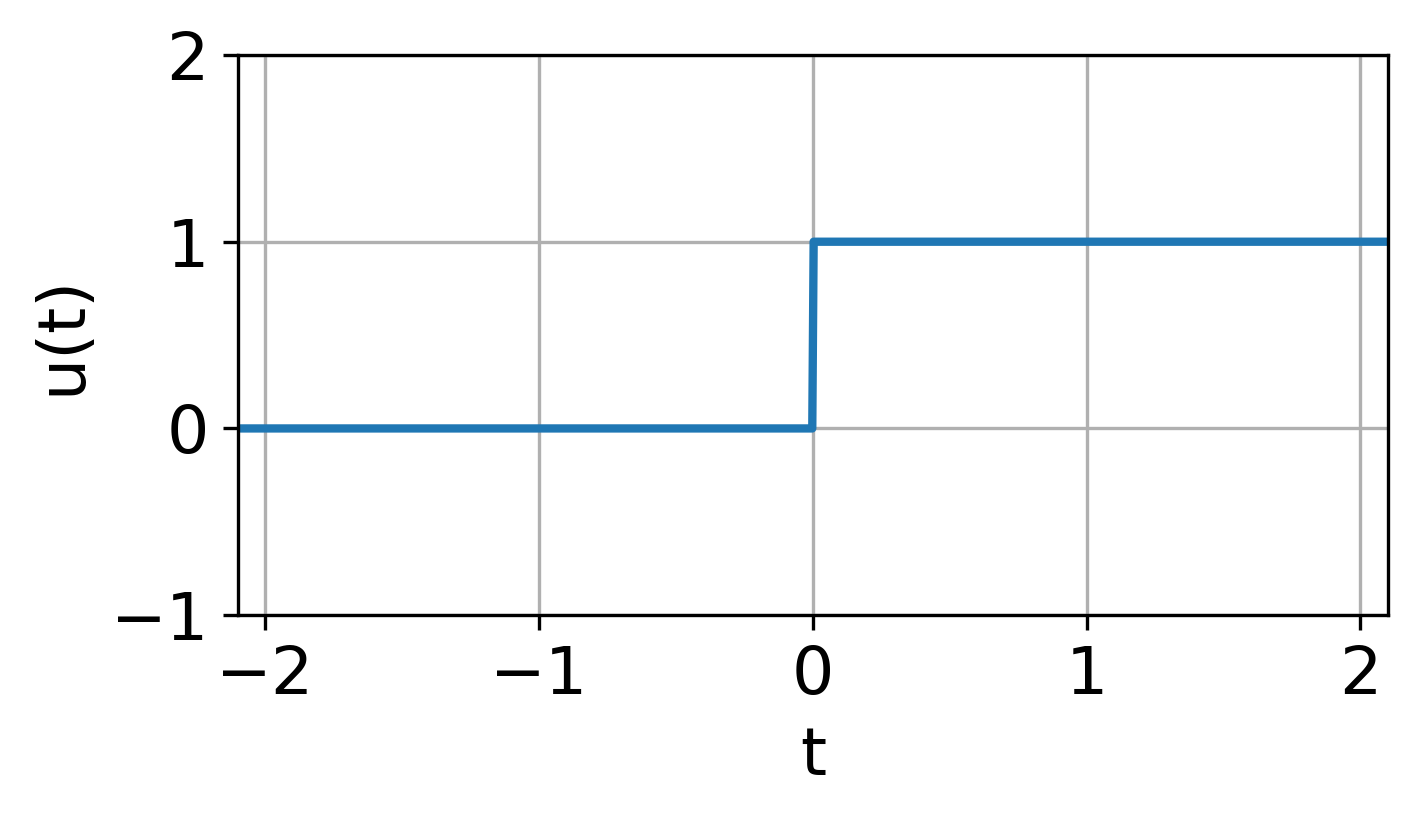
\includegraphics[width=\textwidth/5]{step_function}
		
		\section{Unit pulse function $\Pi(t)$.}
		Describes something lasting for one second and centred at $t=0$:
			\begin{equation*}
				\Pi(t) = \begin{cases}
					1 &\text{for}~\lvert t \rvert \leq \frac{1}{2}\\
					0 &\text{elsewhere}
				\end{cases}
			\end{equation*}
		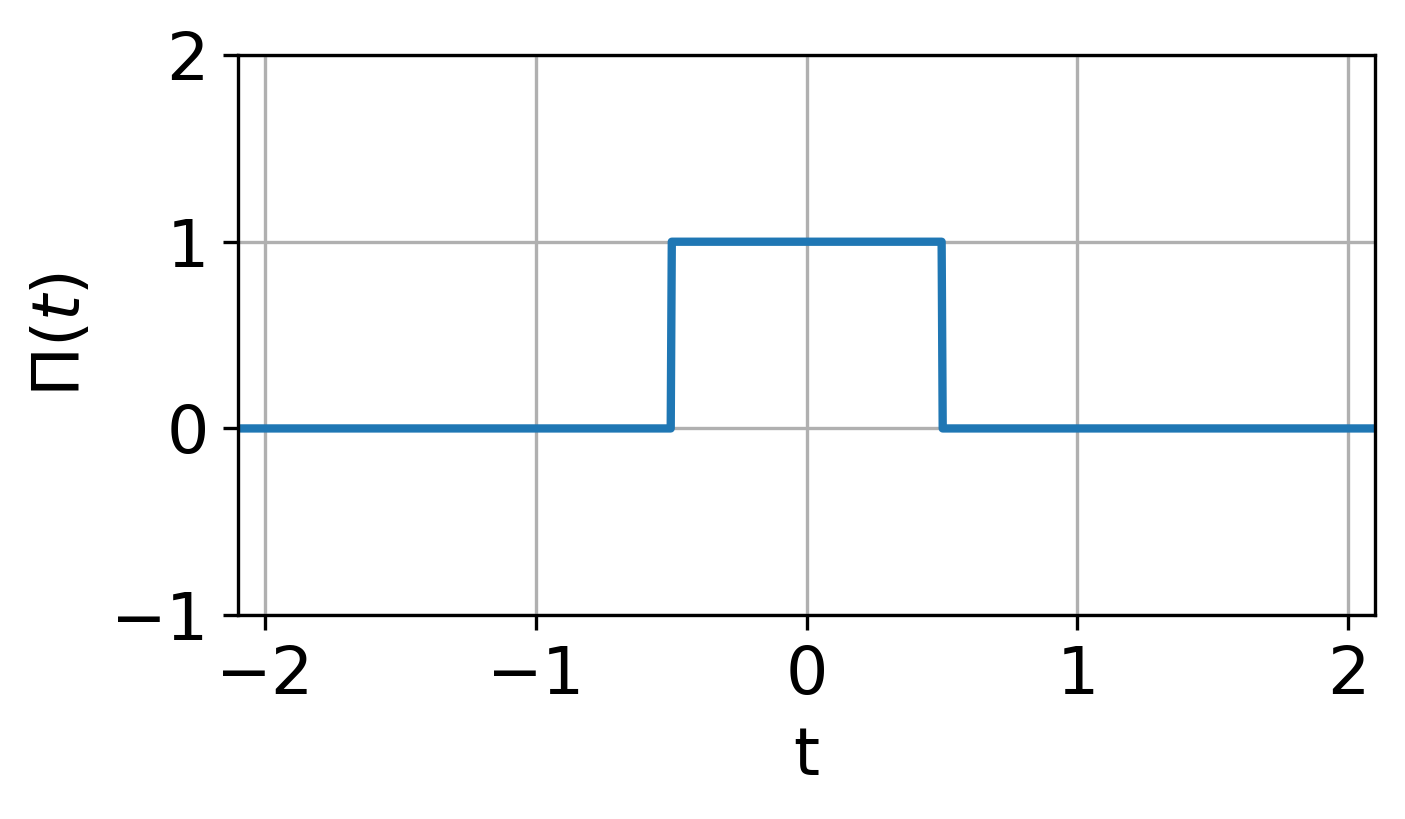
\includegraphics[width=\textwidth/5]{unitpulse_function}
		
		\section{Discrete-time unit impulse $\delta[n]$.}
		Describes something lasting for one sample and centred at $n=0$:
			\begin{equation*}
				\delta[n] = \begin{cases}
					1 &\text{for}~n=0\\
					0 &\text{elsewhere}
				\end{cases}
			\end{equation*}
		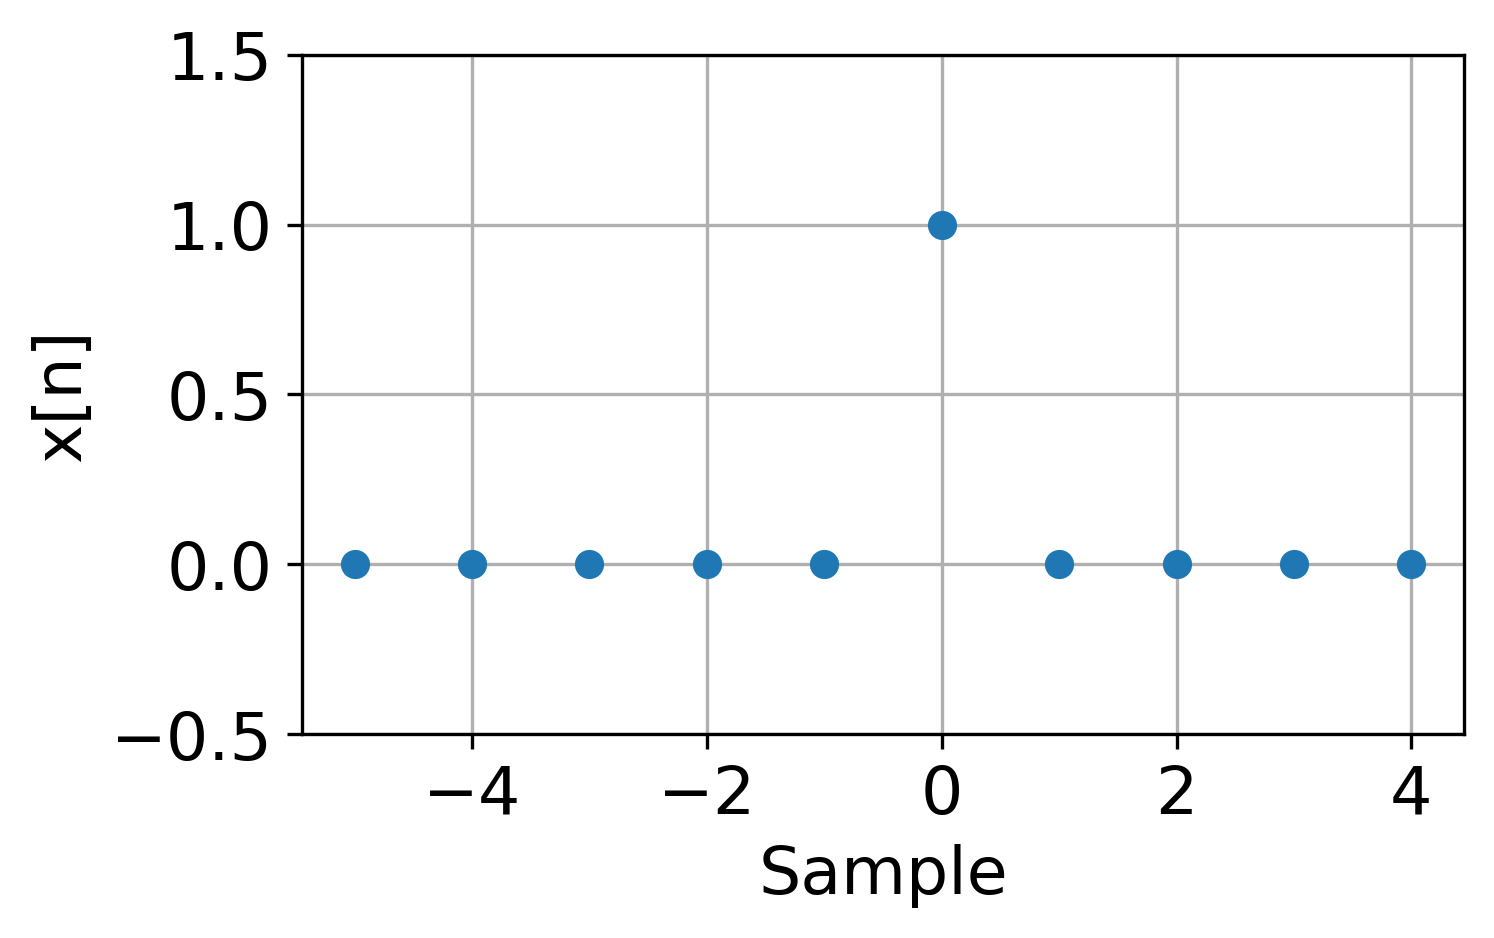
\includegraphics[width=\textwidth/5]{discrete_impulse}
		
		\section{Sinc function $\sinc(t)$.}
			\begin{equation*}
				\sinc(t) = \frac{\sin{(\pi \cdot t)}}{\pi \cdot t}
			\end{equation*}
		Sampling the $\sinc$ function with sampling intervals $T_s = 1$ gives us the discrete unit pulse $\delta[n] = \sinc(1 \cdot n)$.
		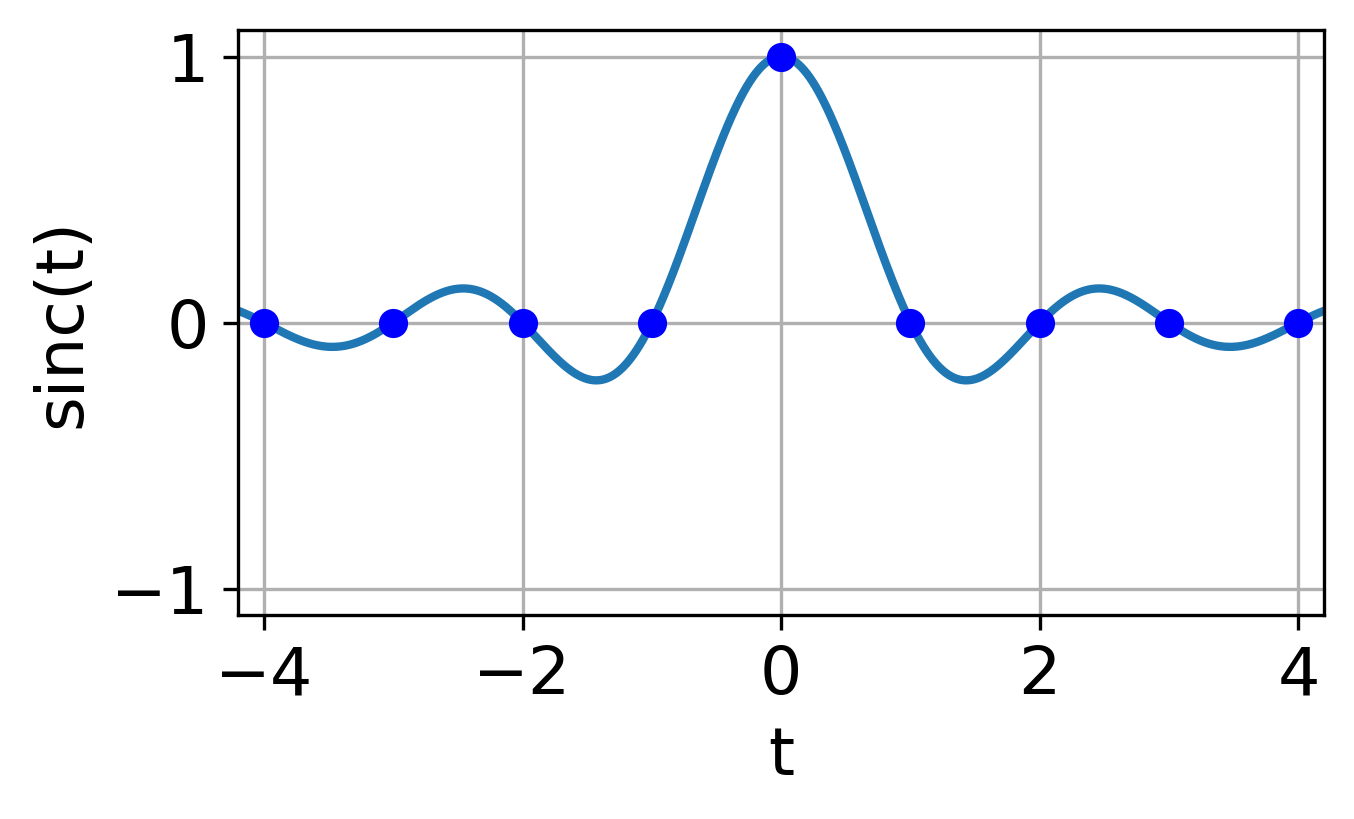
\includegraphics[width=\textwidth/5]{sinc_sampled}
		
		\section{Periodic signals.}
		Periodic signals repeat after period $T_0 = \frac{1}{f_0} = \frac{2\pi}{\omega_0}$:
			\begin{equation*}
				x(t) = x(t + T_0) = x(t + n \cdot T_0)
			\end{equation*}
		
		\section{Phasors.}
		Take
			\begin{equation*}
				x(t) = 2 \cdot \cos{\left(2\pi \cdot 10 \cdot t + \frac{\pi}{4}\right)}
			\end{equation*}
		Using Euler's theorem:
			\begin{equation*}
				x(t) = \Re{\left(2 \cdot e^{j(2\pi \cdot 10 \cdot t + \frac{\pi}{4})}\right)} = \frac{1}{2} \left(2 \cdot e^{j(2\pi \cdot 10 \cdot t + \frac{\pi}{4})} + 2\cdot e^{-j (2\pi \cdot 10 \cdot t + \frac{\pi}{4})}\right)
			\end{equation*}
		
		\section{Dirac delta function $\delta(t)$.}
		Properties that define it:
			\begin{equation*}
				\delta(t) = 0~\text{for}~t \neq 0
			\end{equation*}
			\begin{equation*}
				\int_{-\infty}^{\infty} \delta(t)~dt = 1
			\end{equation*}
		Consequences:
			\begin{equation*}
				u(t) = \int_{-\infty}^{t} \delta(\tau)~d\tau
			\end{equation*}
			\begin{equation*}
				\int_{-\infty}^{\infty} x(\tau) \cdot \delta(t - \tau)~d\tau = \int_{-\infty}^{\infty} x(t - \tau) \cdot \delta(\tau)~d\tau= x(t)
			\end{equation*}
		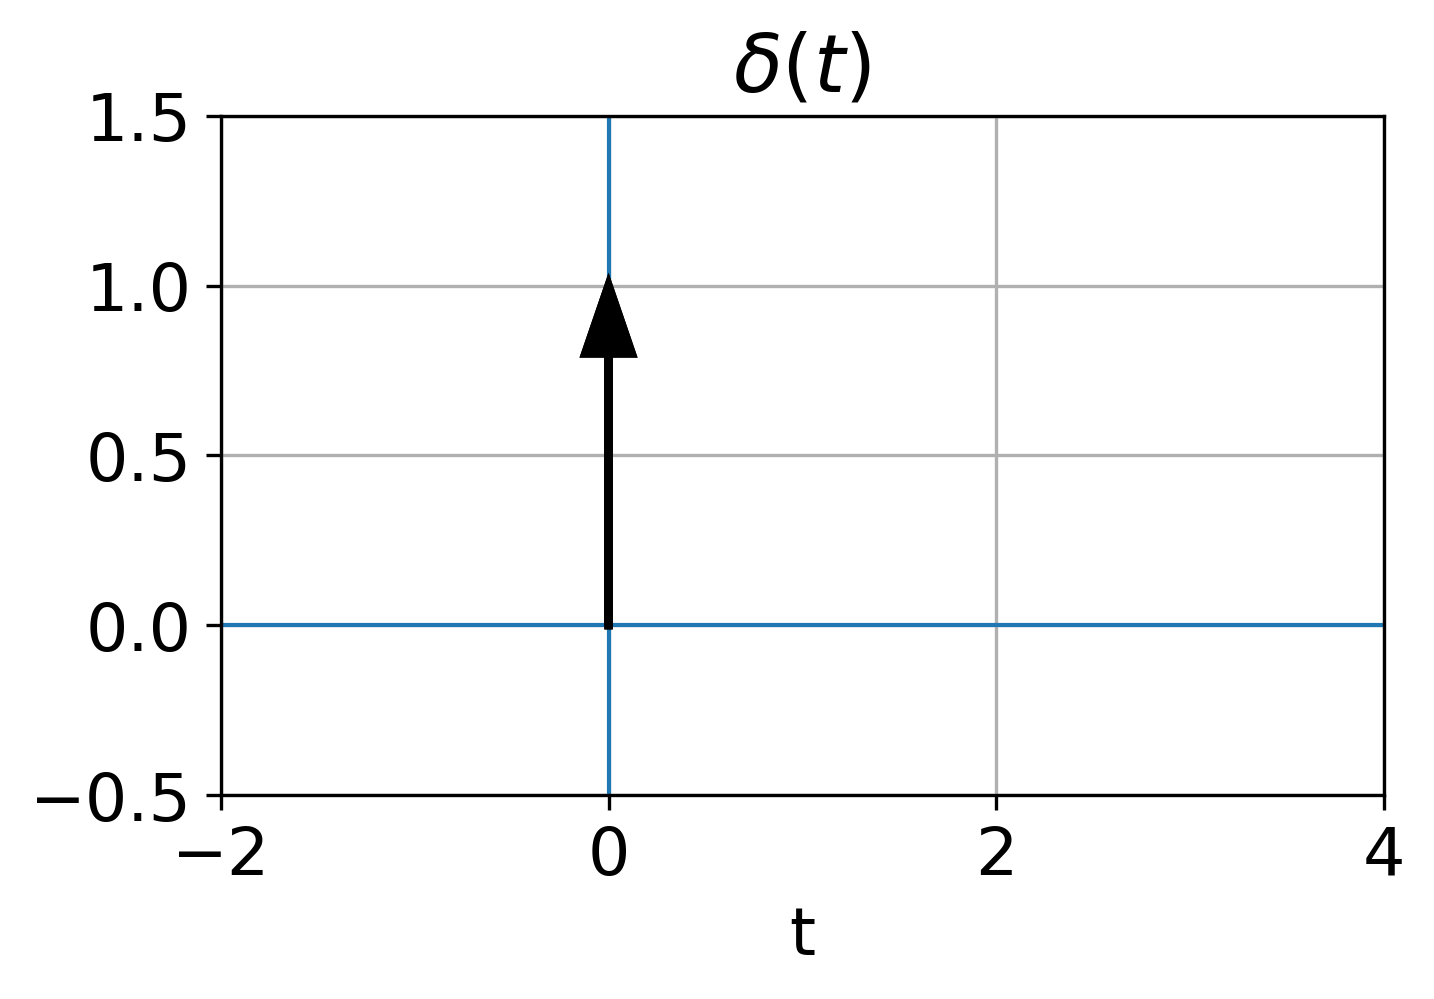
\includegraphics[width=\textwidth/5]{delta_0}
		
		\section{Energy and power of a signal.}
			\begin{equation*}
				E = \int_{-\infty}^{\infty} {\lvert x(t) \rvert}^2~dt
			\end{equation*}
		Formally it is
			\begin{equation*}
				E = \lim_{T \rightarrow \infty} \int_{-T/2}^{T/2} {\lvert x(t) \rvert}^2~dt
			\end{equation*}
		For signals with infinite energy:
			\begin{equation*}
				P = \lim_{T \rightarrow \infty} \frac{1}{T} \int_{-T/2}^{T/2} {\lvert x(t) \rvert}^2~dt
			\end{equation*}
		For periodic signals:
			\begin{equation*}
				P = \frac{1}{T_0} \int_{<T_0>} {\lvert x(t) \rvert}^2~dt
			\end{equation*}
		
		\section{Systems defined by simple ODEs.}
		For a system described by
			\begin{equation*}
				\frac{dy(t)}{dt} + k \cdot y(t) = k \cdot x(t)
			\end{equation*}
		where $x(t) = T_0~u(t)$, the solution $y(t)$ is given by
			\begin{equation*}
				y(t) = T_0 \left(1 - e^{-kt}\right) \cdot u(t)
			\end{equation*}
		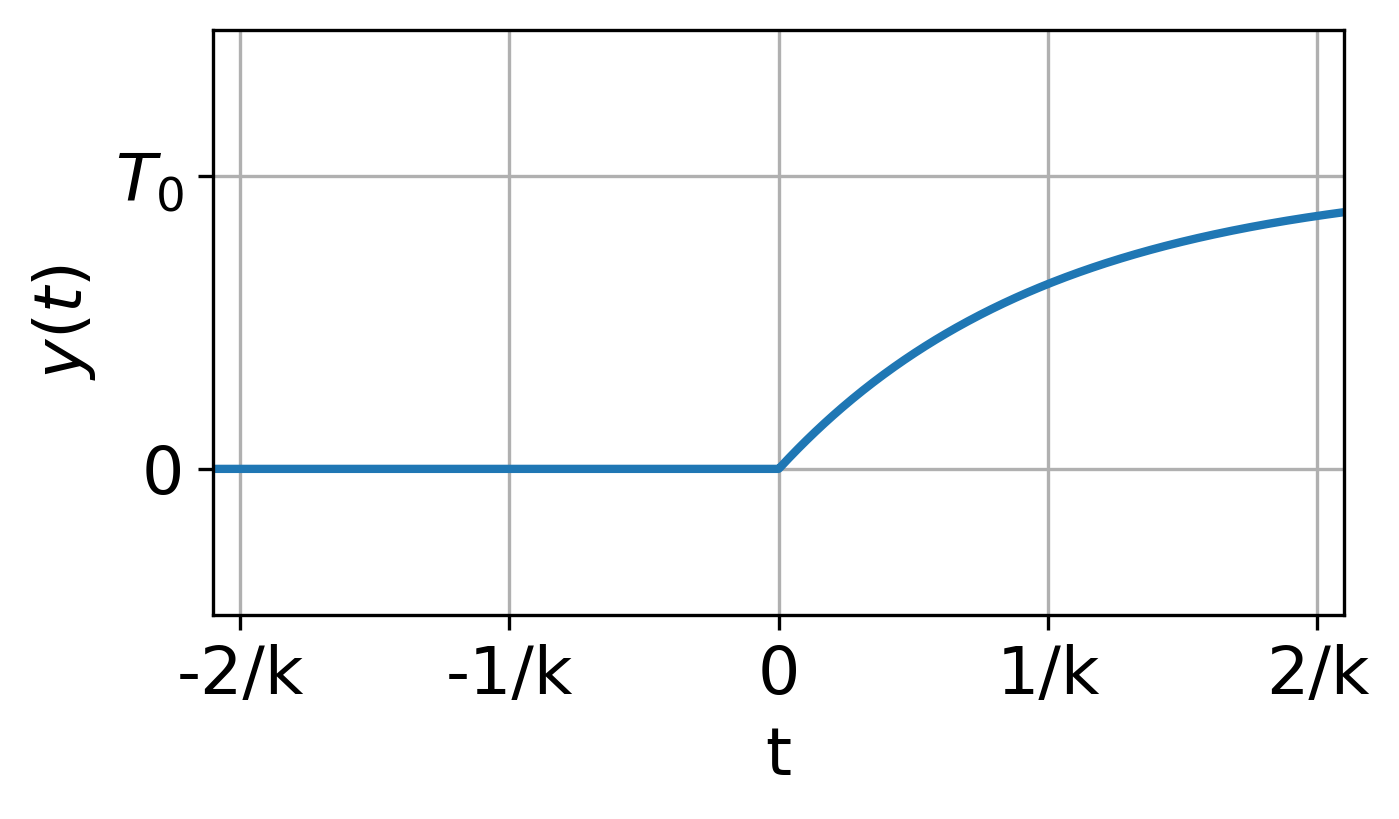
\includegraphics[width=\textwidth/5]{thermo_step_response}
		
		The output of a system where the input is $\delta(n)$ is called the impulse response $h(t)$. In this case:
			\begin{equation*}
				y(t) = h(t) = k \cdot e^{-kt} \cdot u(t)
			\end{equation*}
		
		\section{Variant vs invariant systems.}
		For a time-invariant system with input-output pair x(t) and y(t) and any time-shift $\tau$:
			\begin{equation*}
				x(t - \tau) \rightarrow \boxed{\text{Time-invariant system}} \rightarrow y(t - \tau)
			\end{equation*}
		
		\section{Example.}
			\begin{equation*}
				y(t) = \frac{1}{T_0} \cdot \int_{t-T_0}^{t} x(\alpha)~d\alpha
			\end{equation*}
		Give the input as signal $x_1 (t) = x(t - \tau)$:
			\begin{equation*}
				y_1 (t) = \frac{1}{T_0} \cdot \int_{t-T_0}^{t} x_1(\alpha)~d\alpha
			\end{equation*}
		Variable change: $\beta = \alpha - \tau$, so that $\alpha = \beta + \tau$ and $d\alpha = d\beta$.\\
		Substitute and change the integration limits:
			\begin{equation*}
				y_1 (t) = \frac{1}{T_0} \cdot \int_{(t - \tau) - T_0}^{(t - \tau)} x(\beta)~d\beta = y(t - \tau)
			\end{equation*}
		
		\section{Linear systems.}
		A system is linear if, for any constants $a$ and $b$ and inputs $x_1(t)$ and $x_2(t)$:
			\begin{equation*}
				\mathcal{H}[a \cdot x_1(t) + b \cdot x_2(t)] = a \cdot \mathcal{H}[x_1(t)] + b \cdot \mathcal{H}[x_2 (t)]
			\end{equation*}
		
		\section{Causal systems.}
		A system is causal if the output signal does not depend on future inputs.\\
		Example: $y(t) = \frac{1}{T_0} \cdot \int_{t-T_0}^{t} x(\alpha)~d\alpha$.\\
		Counter-example: $\mathcal{H}[x(t)] = x(t + 1)$, $\mathcal{H}[x(t)] = \frac{1}{T_0} \cdot \int_{t}^{t+T_0} x(\alpha)~d\alpha$.
		
		\section{LTI systems, impulse response, and the convolution.}
			\begin{equation*}
				\delta(t) \rightarrow \boxed{\text{System}} \rightarrow h(t)
			\end{equation*}
			\begin{equation*}
				x(t) \rightarrow \boxed{\text{System}} \rightarrow \int_{-\infty}^{\infty} x(\tau) \cdot h(t - \tau)~d\tau = x(t) * h(t)
			\end{equation*}
		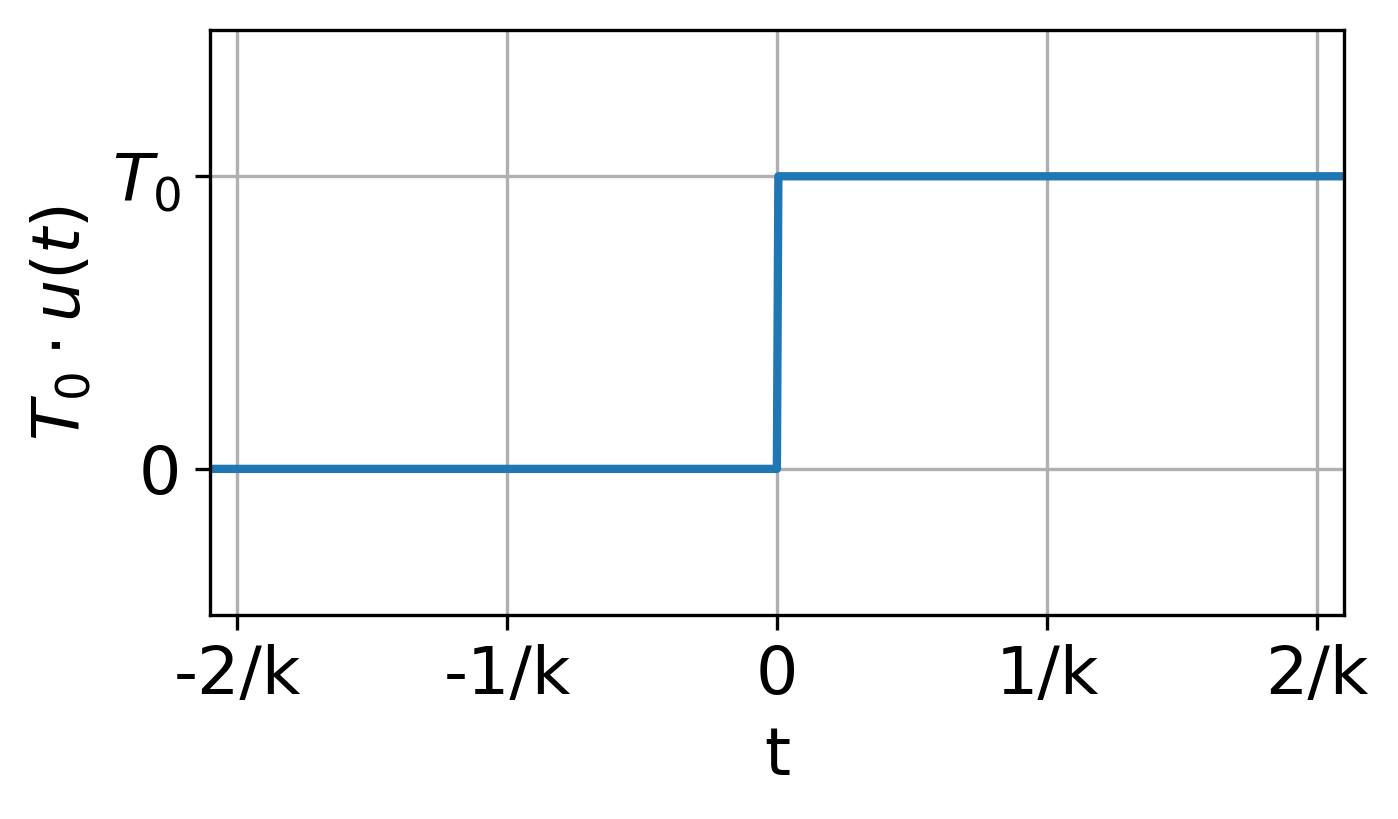
\includegraphics[width=\textwidth/5]{step_temperature}
		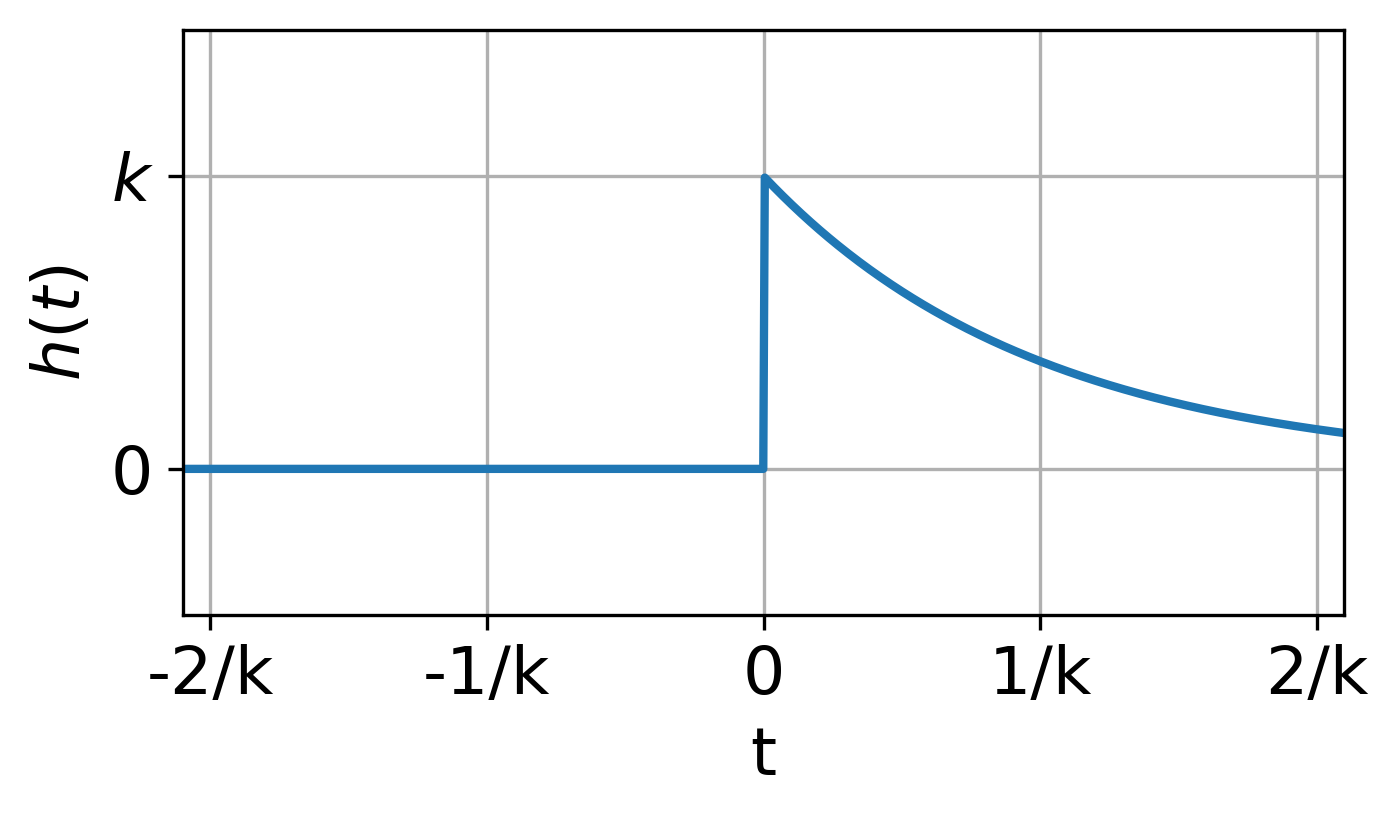
\includegraphics[width=\textwidth/5]{thermo_impulse_response}
		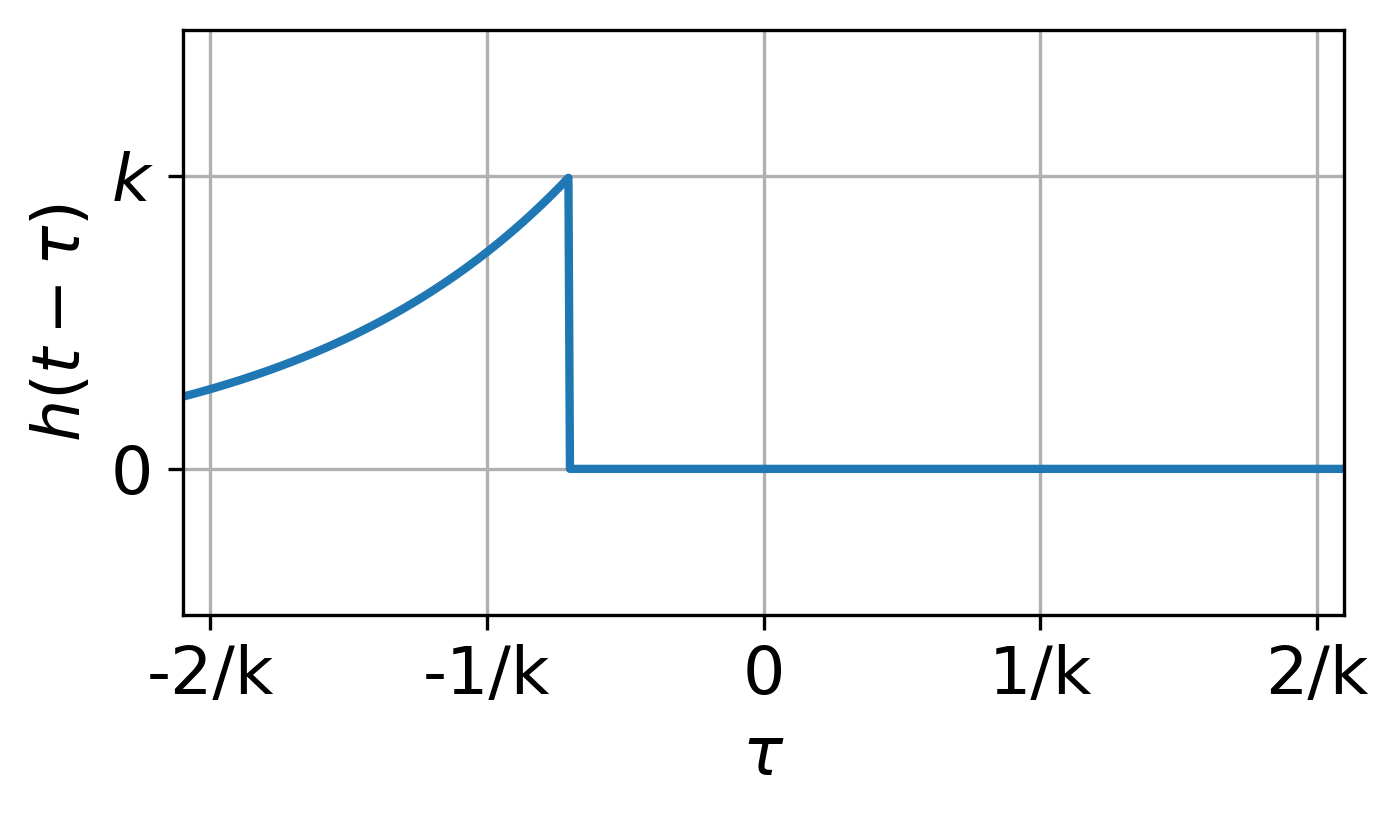
\includegraphics[width=\textwidth/5]{thermo_impulse_response_reversed_case1}
		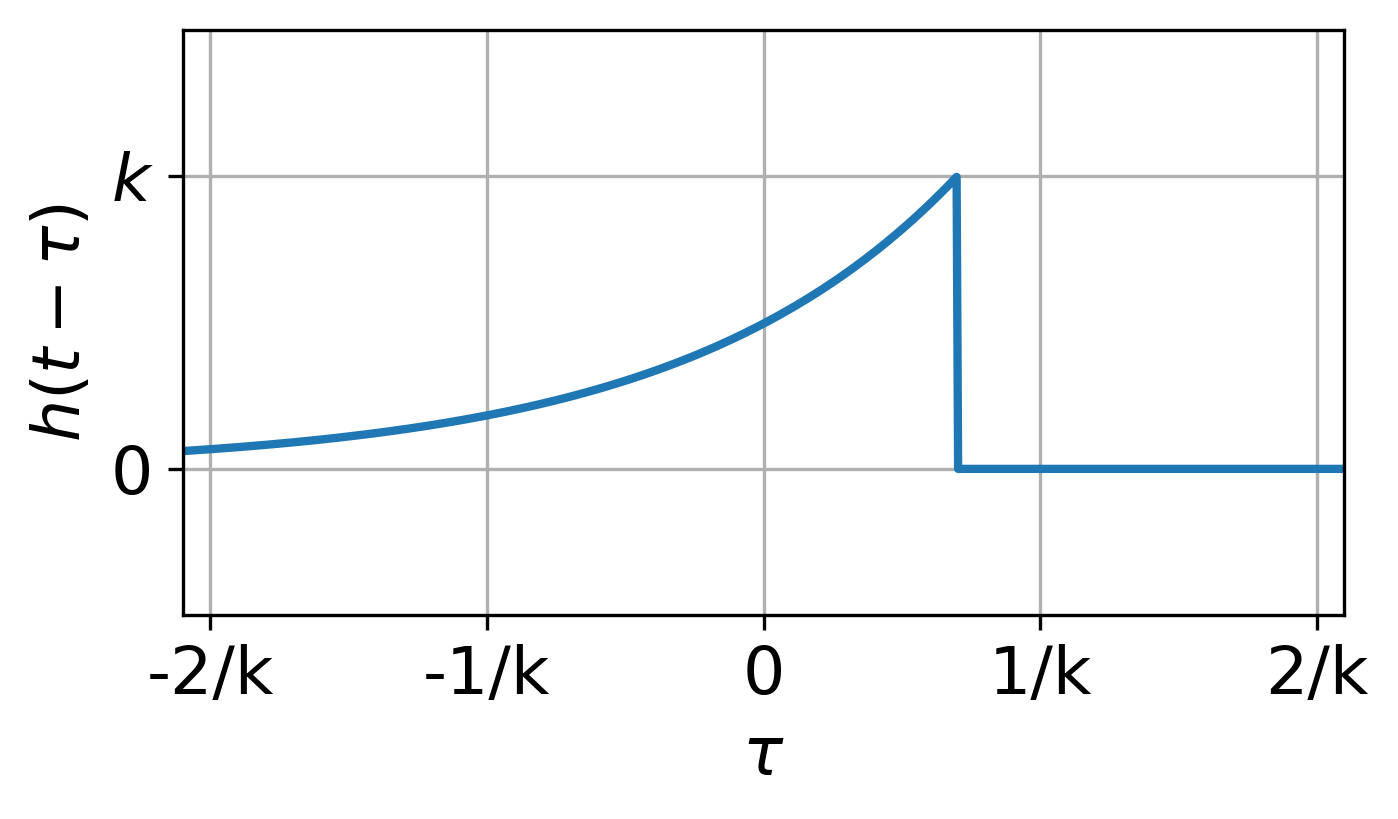
\includegraphics[width=\textwidth/5]{thermo_impulse_response_reversed_case2}
		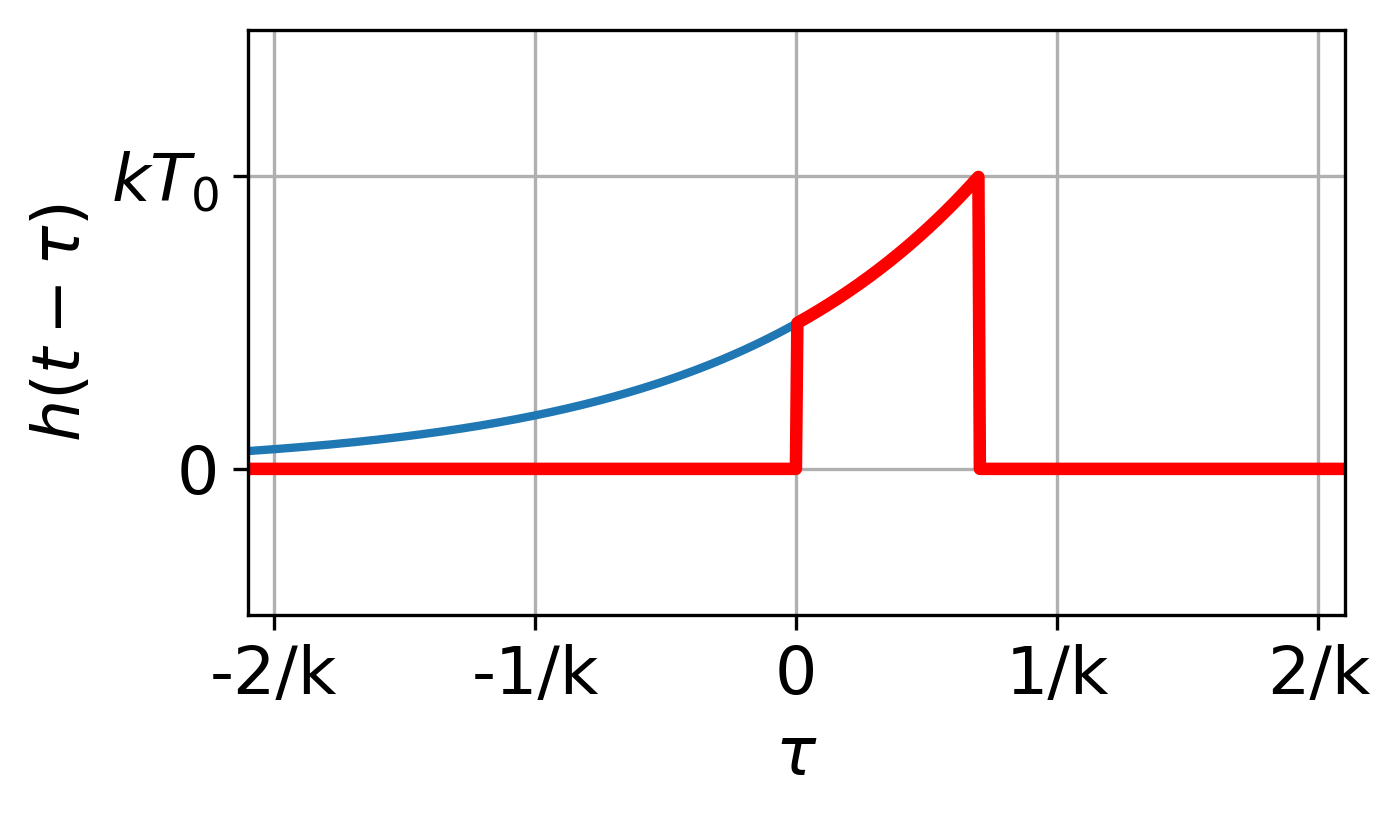
\includegraphics[width=\textwidth/5]{thermo_impulse_response_reversed_case2b}
		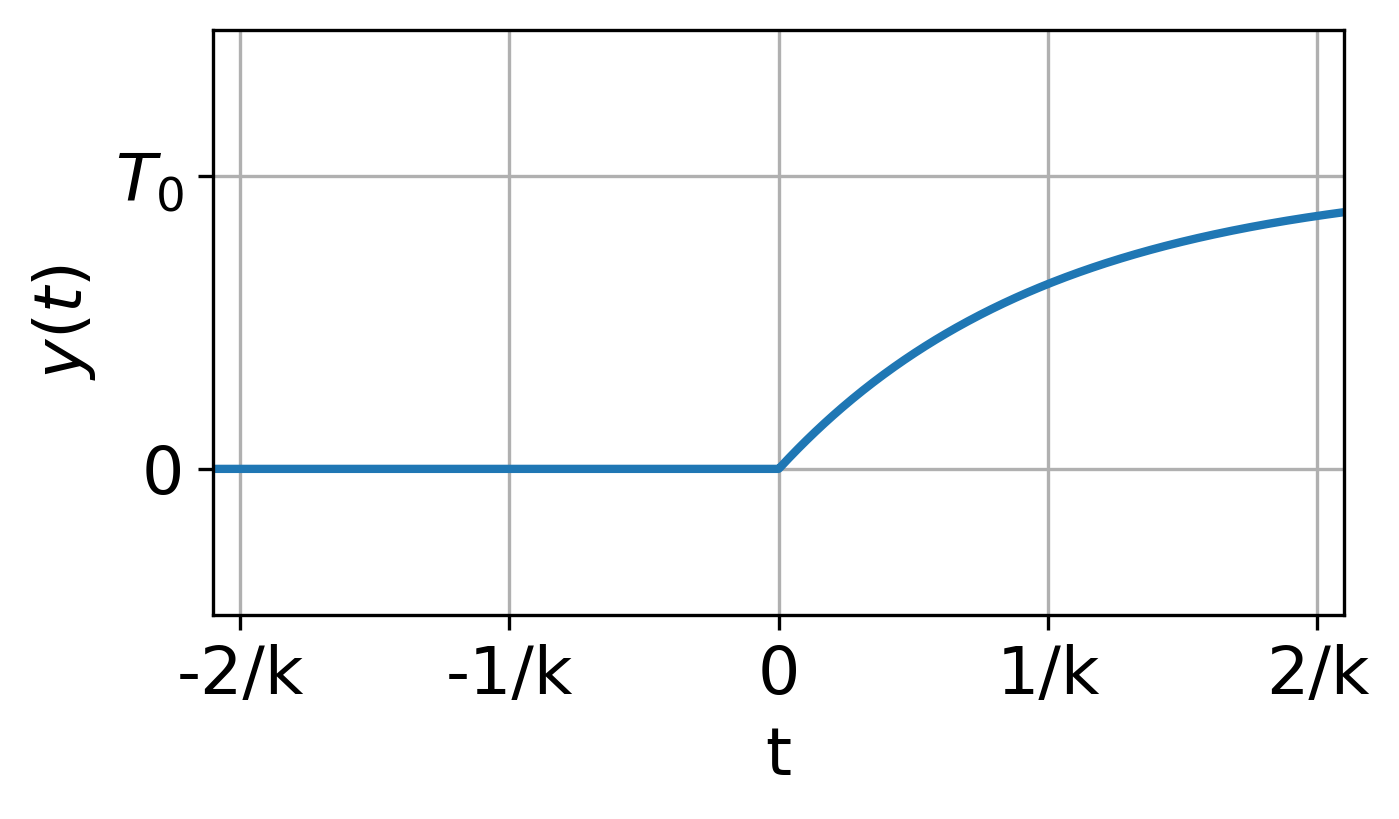
\includegraphics[width=\textwidth/5]{thermo_step_response}\\
		Temporal length of the output = length of input + length of $h(t)$.
		
		\section{Properties of the convolution.}
		Commutative: $x(t) * y(t) = y(t) * x(t)$\\
		Associative: $x(t) * h_1(t) * h_2(t) = x(t)*(h_1(t)*h_2(t))$\\
		Distributive: $x(t) * h_1(t) + x(t) * h_2(t) = x(t)*(h_1(t)+h_2(t))$
		
		\section{Frequency response.}
			\begin{equation*}
				x(t) = e^{j 2\pi f_0 t} \rightarrow \boxed{\text{H(f)}} \rightarrow e^{j 2\pi f_0 t} \cdot H(f_0)
			\end{equation*}
			\begin{equation*}
				\begin{split}
					x(t) * h(t) & = \int_{-\infty}^{\infty} h(\tau) \cdot e^{j 2\pi f_0 (t-\tau)}~d\tau \\
					& = e^{j 2\pi f_0 t} \int_{-\infty}^{\infty} h(\tau) \cdot e^{- j 2\pi f_0 \tau}~d\tau
				\end{split}
			\end{equation*}
		$H(f)$: frequency response. The frequency response is the Fourier transform of the impulse response.
			\begin{equation*}
				H(f) = \int_{-\infty}^{\infty} h(\tau) \cdot e^{-j2\pi f \tau}~d\tau = \int_{-\infty}^{\infty} h(t) \cdot e^{-j2\pi ft}~dt
			\end{equation*}
		
		\section{Constructing periodic signals.}
			\begin{equation*}
				x_0(t) = a_0 + \sum_{k=1}^{n} a_k \cos(k \omega_0 t) + \sum_{k=1}^{n} b_k \sin(k \omega_0 t)
			\end{equation*}
			\begin{equation*}
				x_0(t) = \sum_{n=-N}^{N} X_n e^{j n \omega_0 t}
			\end{equation*}
		
		\section{Synthesis and analysis equations.}
		A non-pathological periodic function with period $T_0$ can be expressed as
			\begin{equation*}
				x(t) = \sum_{n=0}^{\infty} a_n \cos(n \omega_0 t) + \sum_{n=1}^{\infty} b_n \sin(n \omega_0 t),
			\end{equation*}
		with\\
		$\qquad a_0 = \frac{1}{T_0} \int_{<T_0>} x(t)~dt = \frac{1}{T_0} \int_{0}^{T_0} x(t)~dt = \frac{1}{T_0} \int_{-T_0/2}^{T_0/2} x(t)~dt$,\\
		$\qquad a_n = \frac{2}{T_0} \int_{<T_0>} x(t) \cdot \cos(n \omega_0 t)~dt$,\\
		$\qquad b_n = \frac{2}{T_0} \int_{<T_0>} x(t) \cdot \sin(n \omega_0 t)~dt$.\\
		$a_0$ is the mean value. $\cos(n \omega_0 t)$ are even functions of $t(x(t) = x(-t))$. $\sin(n \omega_0 t)$ are odd functions of $t(x(t) = -x(-t))$.
		
		\section{Complex Fourier series.}
		Since
			\begin{equation*}
				\cos(n \omega_0 t) = \frac{1}{2} e^{-j n \omega_0 t} + \frac{1}{2} e^{j n \omega_0 t}
			\end{equation*}
			and
			\begin{equation*}
				\sin(n \omega_0 t) = \frac{j}{2} e^{-j n \omega_0 t} - \frac{j}{2} e^{j n \omega_0 t},
			\end{equation*}
		we can rewrite the Fourier series as
			\begin{equation*}
				x(t) = \sum_{n=0}^{\infty} a_n \cos(n \omega_0 t) + \sum_{n=1}^{\infty} b_n sin(n \omega_0 t) = \sum_{n=-\infty}^{\infty} X_n \cdot e^{j n \omega_0 t}
			\end{equation*}
		with
			\begin{equation*}
				X_n = \frac{1}{T_0} \int_{<T_0>} x(t) \cdot e^{-j n \omega_0 t}~dt
			\end{equation*}
		
		\section{Symmetry property.}
		For real-valued signals:
			\begin{equation*}
				X_n = X_{-n}^*
			\end{equation*}
		Real part is even function of $n$.\\
		Imaginary part is odd function of $n$.\\
		Amplitude $\lvert X_n \rvert$ is even function.\\
		Phase is odd.
		
		\section{Differentiation.}
			\begin{equation*}
				x(t) \rightarrow \boxed{\frac{d}{dt}} \rightarrow \mathcal{H}[x(t)] = \frac{dx(t)}{dt} = \dot{x}(t)
			\end{equation*}
		Per definition:
			\begin{equation*}
				h(t) = \dot{\delta}(t)
			\end{equation*}
		Thus:
			\begin{equation*}
				\mathcal{H}[x(t)] = x(t) * \dot{\delta}(t) = \int_{-\infty}^{\infty} x(\tau) \cdot \dot{\delta}(t - \tau)~dt = \dot{x}(t)
			\end{equation*}
			\begin{equation*}
				e^{jk\omega_0 t} \rightarrow \boxed{\frac{d}{dt}} \rightarrow jk\omega_0 \cdot e^{jk\omega_0 t}
			\end{equation*}
			\begin{equation*}
				X_l e^{jl\omega_0 t} + X_k e^{jk\omega_0 t} \rightarrow \boxed{\frac{d}{dt}} \rightarrow jl\omega_0 X_l e^{jl\omega_0 t} + jk\omega_0 X_k e^{jk\omega_0 t}
			\end{equation*}
			\begin{equation*}
				\sum_{k=-\infty}^{\infty} X_k e^{jk\omega_0 t} \rightarrow \boxed{\frac{d}{dt}} \rightarrow \sum_{k=-\infty}^{\infty} jk\omega_0 X_k e^{jk\omega_0 t}
			\end{equation*}
		Thus the derivative of a complex Fourier series is another one with new coefficients
			\begin{equation*}
				X_k^{\prime} = jk\omega_0 X_k
			\end{equation*}
		
		\section{Response of LTI system to periodic signal.}
			\begin{equation*}
				\sum_{k=-\infty}^{\infty} X_k e^{jk\omega_0 t} \rightarrow \boxed{\begin{matrix}h(t)\\H(\omega)\end{matrix}} \rightarrow \sum_{k=-\infty}^{\infty} H(k\omega_0) \cdot X_k e^{jk\omega_0 t}
			\end{equation*}
			\begin{equation*}
				\tilde{X}_k = H(k\omega_0) \cdot X_k
			\end{equation*}
		
		\section{Parseval's theorem.}
			\begin{equation*}
				\begin{split}
					P &= \frac{1}{T_0} \int_{0}^{T_0} {\lvert x(t) \rvert}^2~dt = \frac{1}{T_0} \int_{0}^{T_0} x(t) \cdot x(t)^*~dt\\
					&= \sum_{n=-\infty}^{\infty} X_n^* \cdot X_n = \sum_{n=-\infty}^{\infty} {\lvert X_n \rvert}^2
				\end{split}
			\end{equation*}
		For trigonometric series:
			\begin{equation*}
				P = \frac{1}{T_0} \int_{0}^{T_0} {\lvert x(t)\rvert}^2~dt = a_0^2 + \frac{1}{2} \sum_{n=1}^{\infty} a_n^2 + \frac{1}{2} \sum_{n=1}^{\infty} b_n^2
			\end{equation*}
		
		\newpage
	\end{multicols}
\end{document}







